\documentclass[a4paper,11pt]{ltjsarticle}
\usepackage{graphicx}
\usepackage{luatexja-fontspec}
\usepackage{caption}
\usepackage{amsmath,amssymb,bm,braket}
\usepackage[english]{babel}
\usepackage{multicol}
\usepackage{titlesec}
%\usepackage{gnuplot-lua-tikz}
\usepackage[top=20truemm,bottom=20truemm,left=20truemm,right=20truemm]{geometry}
\usepackage{array}
\usepackage{upgreek}
\usepackage{fancyhdr}
\renewcommand{\refname}{}
\usepackage{listings,jvlisting}
\usepackage{tikz}
\usepackage[thmmarks,amsmath]{ntheorem}
\usepackage[version=3]{mhchem}
\usetikzlibrary{external}
\tikzexternalize
\lstset{
  basicstyle={\ttfamily},
  identifierstyle={\small},
  commentstyle={\smallitshape},
  keywordstyle={\small\bfseries},
  ndkeywordstyle={\small},
  stringstyle={\small\ttfamily},
  frame={tb},
  breaklines=true,
  columns=[l]{fullflexible},
  numbers=left,
  xrightmargin=0pt,
  xleftmargin=3pt,
  numberstyle={\scriptsize},
  stepnumber=1,
  numbersep=1pt,
  lineskip=-0.5ex
}
\captionsetup[figure]{format=plain, labelformat=simple, labelsep=quad,labelfont=bf,name={Fig.}}
\captionsetup[table]{format=plain, labelformat=simple, labelsep=quad,labelfont=bf}
\parindent = 0pt
%[BoldFont=HGSMinchoE]{MSMincho}[BoldFont=HiraMinProN-W6]{HiraMinPro-W3}
\titleformat{\section}{\normalfont\fontsize{9}{10}\bfseries\fontspec{Times New Roman}}{\thesection.}{1em}{}
\usepackage[backend=biber,sorting=none,style=numeric,maxnames=99,minnames=1]{biblatex}
\addbibresource{utility/REFERENCES.bib}
\defbibheading{bibliography}[\refname]{%
  \section*{REFERENCES}%
  \vspace{-7pt}  % ここで空白を調整。お好みの値に変更してください。
}
\newfontfamily\subsectionfont{Times New Roman} % サブセクション用フォント
\titleformat{\subsection}
  {\normalfont\large\bfseries} % サブセクションのフォントを指定
  {\thesubsection}{1em}{}
\renewbibmacro{in:}{}
\renewbibmacro*{journal+issuetitle}{%
  \addcomma\space% カンマとスペースを追加
  \usebibmacro{journal}%
  \setunit*{\addspace}%
  \usebibmacro{volume+number+eid}%
  \setunit{\addspace}%
  \printfield{note}%
  \newunit
}
\renewbibmacro*{volume+number+eid}{
  \printfield{volume}%
  \setunit*{\addnbspace}%
  \printfield{number}%
  \setunit{\addcomma\space}%
  \printfield{eid}
}
\DeclareFieldFormat[article]{volume}{\textbf{#1}}
\DeclareFieldFormat[article]{pages}{#1}
\DeclareFieldFormat{journaltitle}{#1}
\usepackage{hyperref}
\renewenvironment{abstract}{\par\noindent}{\par}
%\pagenumbering{gobble}
\usepackage{docmute}
\usepackage{setspace}
\usepackage{titlesec} % 見出しのカスタマイズ用

% セクションのフォーマットをカスタマイズ
\titleformat{\section}
  {} % フォントサイズとスタイル
  {\Large\bfseries\thesection\ \ }               % 番号の前の内容(空白)
  {0em}            % 番号とタイトルの間の間隔
  {\Large\bfseries}


\theoremstyle{plain}
\theoremheaderfont{\normalfont\bfseries}
\theorembodyfont{\itshape}   % 本文を斜体に
\theoremseparator{.}         % タイトルと本文の区切りを「.」に設定
\newtheorem{definition}{Definition}
\begin{document}
\section{Results}\label{results}{
    \ \ \ Firstly, we perform numerical simulations of the pseudo-3D Surface Code, introduced in Section~\ref{pseudo-three-dimensional_surface_code}, using a circuit that executes a 2D Heisenberg model and compare it to the 2D Surface Code. The results are presented in Fig.~\ref{results_of_pseudo_3D}, and a more complex system is shown in Fig.~\ref{results_of_pseudo_3D_1}. In these figures, the horizontal and vertical axes represent the instruction number and distance, respectively, where distance refers to the number of patches required for routing operations. Additionally, the 20 magic patches that produce T gates are aligned along $x = -1$, arranged from $y = 0$ to $y = 19$. The Breadth-First Search algorithm is used for routing in the following cases.

    \begin{figure}[h]
        \centering
        \includegraphics[scale=0.5]{figure/results_pseudo_3D.eps}
        \vspace{-20pt}\caption{Results of executing the 2D Heisenberg model circuit in (left) a 2D surface code and (right) a pseudo-3D surface code. The averages are 8.18 for the 2D surface code and 5.36 for the pseudo-3D surface code.}
        \label{results_of_pseudo_3D}
    \end{figure}

    \ \ \ In Fig.~\ref{results_of_pseudo_3D}, the graph illustrates that in the 2D Surface Code, a substantial number of operations exceeded a distance of 30. In contrast, in the 3D Surface Code, the longest operation distance remained below 30. Furthermore, the average distance per operation was significantly reduced from 8.18 in the 2D configuration to 5.36 in the pseudo-3D configuration, resulting in an approximately 66\% improvement in overall circuit distance. However, the total time required to execute the entire circuit did not change despite expanding the routing dimension to pseudo-3D.

    \begin{figure}[h]
        \centering
        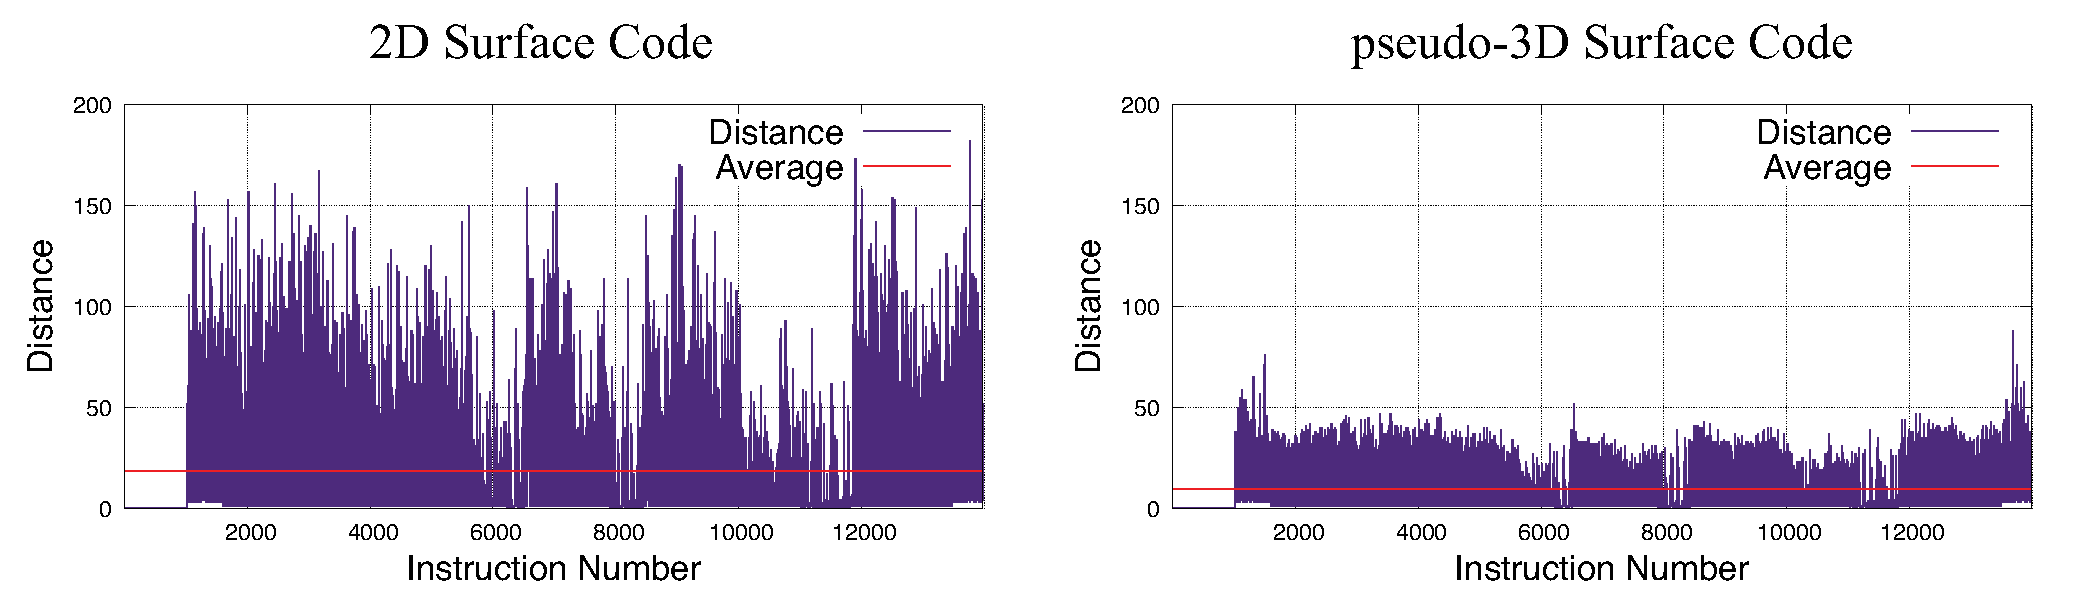
\includegraphics[scale=0.5]{figure/results_pseudo_3D_1.eps}
        \vspace{-20pt}\caption{Results of executing a more complex 2D Heisenberg model circuit in (left) a 2D surface code and (right) a pseudo-3D surface code. The averages are 18.64 for the 2D surface code and 9.74 for the pseudo-3D surface code.}
        \label{results_of_pseudo_3D_1}
    \end{figure}

    In the more complex circuit, where the Heisenberg model system is the same as in the former case but is more parallelized and thus requires more ancilla qubits, similar improvements are observed, as shown in Fig.~\ref{results_of_pseudo_3D_1}. This further demonstrates the effectiveness of the pseudo-3D Surface Code in reducing operation distances. The average distance per operation was significantly reduced from 18.64 in the 2D configuration to 9.74 in the pseudo-3D configuration, resulting in an approximately 52\% improvement in overall circuit distance. However, the total time required to execute the entire circuit did not change in the more complex system. Therefore, the pseudo-3D Surface Code does not improve the parallelization of the circuit.\\
    \ \ \ Secondly, we perform numerical simulations of the placement optimization method introduced in Section~\ref{placement_optimization}. The results are presented in Fig.~\ref{placement_optimization_2D} for the 2D case and Fig.~\ref{placement_optimization_3D} for the pseudo-3D case. Additionally, the graphs optimized by the potential energy model are shown in Fig.~\ref{graph_2D} and Fig.~\ref{graph_3D}. Each figure in Figs.~\ref{placement_optimization_2D}--\ref{graph_3D} displays the results of a smaller circuit in the top row and a larger circuit in the bottom row. The system for the Heisenberg model is the same as in the previous case; thus, the results on the left-hand side of Figs.~\ref{placement_optimization_2D}--\ref{graph_3D} have already been discussed in the preceding paragraph. The 20 magic patches that produce T gates are aligned along $x = -1$, arranged from $y = 0$ to $y = 19$, while logical patches are allocated in the range of $x \geq 0$ and $y \geq 0$. The parameter $l$, introduced in Section~\ref{placement_optimization}, was tuned to a value of 3 in all the following cases, and the Breadth-First Search (BFS) algorithm is used for routing in the following cases.

    \begin{figure}[h]
        \centering
        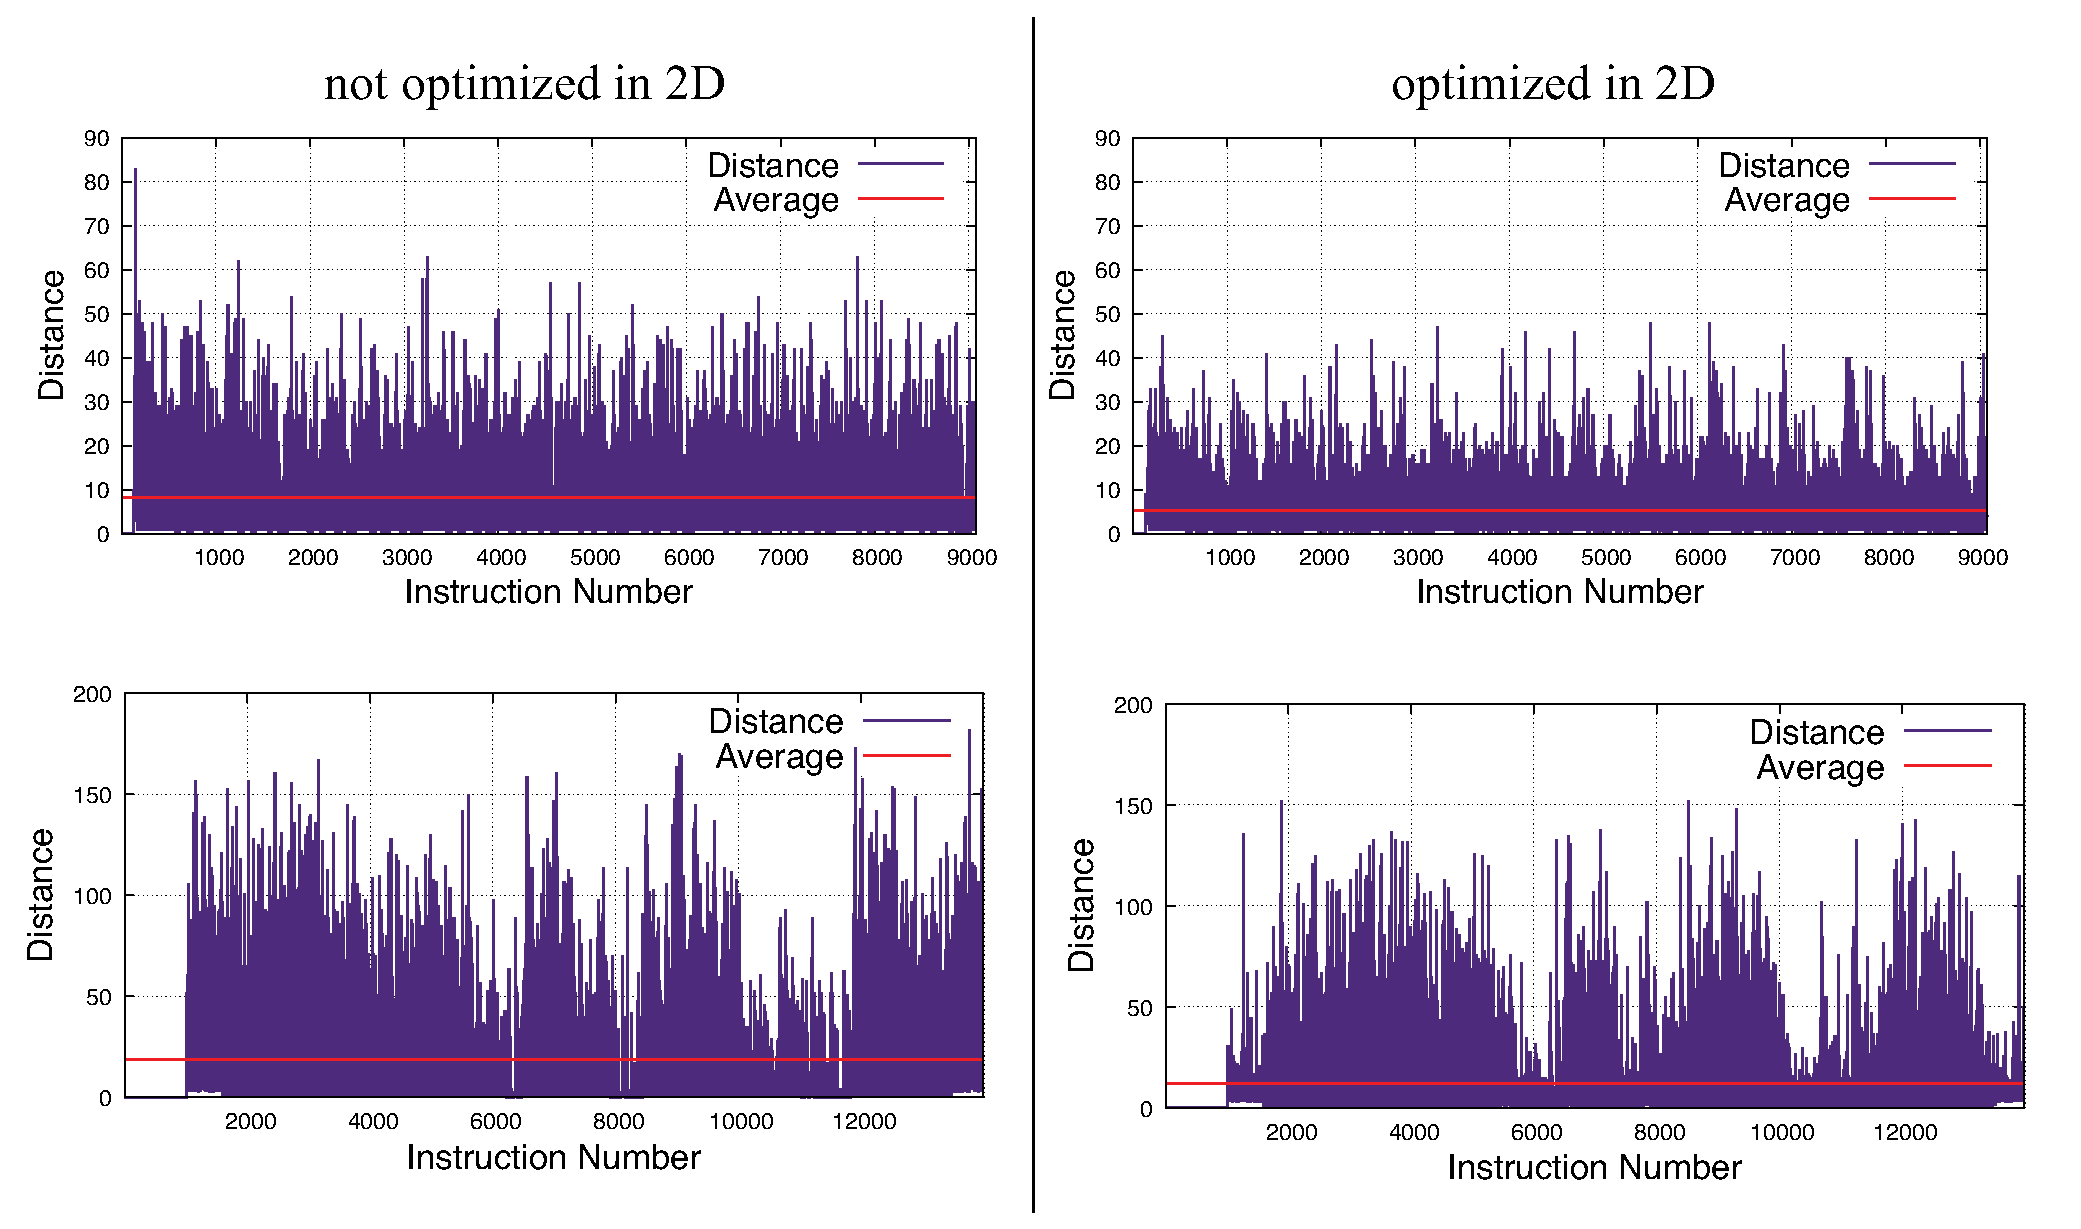
\includegraphics[scale=0.5]{figure/placement_optimization_2D.eps}
        \vspace{-20pt}\caption{Results of placement optimization for executing the 2D Heisenberg model circuit. (Left) Unoptimized cases in 2D surface codes. (Right) Optimized cases in 2D surface codes. Additionally, the bottom rows present results for more complex circuits compared to the top rows. The average values are 8.18 (left top), 5.18 (right top), 18.64 (left bottom), and 12.15 (right bottom).}
        \label{placement_optimization_2D}
    \end{figure}

    \vspace{-5pt}
    \ \ \ In Fig.~\ref{placement_optimization_2D}, we obtained results showing that placement optimization decreases routing distances. Specifically, the average distance in the 2D optimized configuration was reduced to 5.18 for the smaller circuit and to 12.15 for the larger circuit, resulting in a 63\% improvement in the smaller circuit and a 65\% improvement in the larger circuit.
    
    \begin{figure}[h]
        \centering
        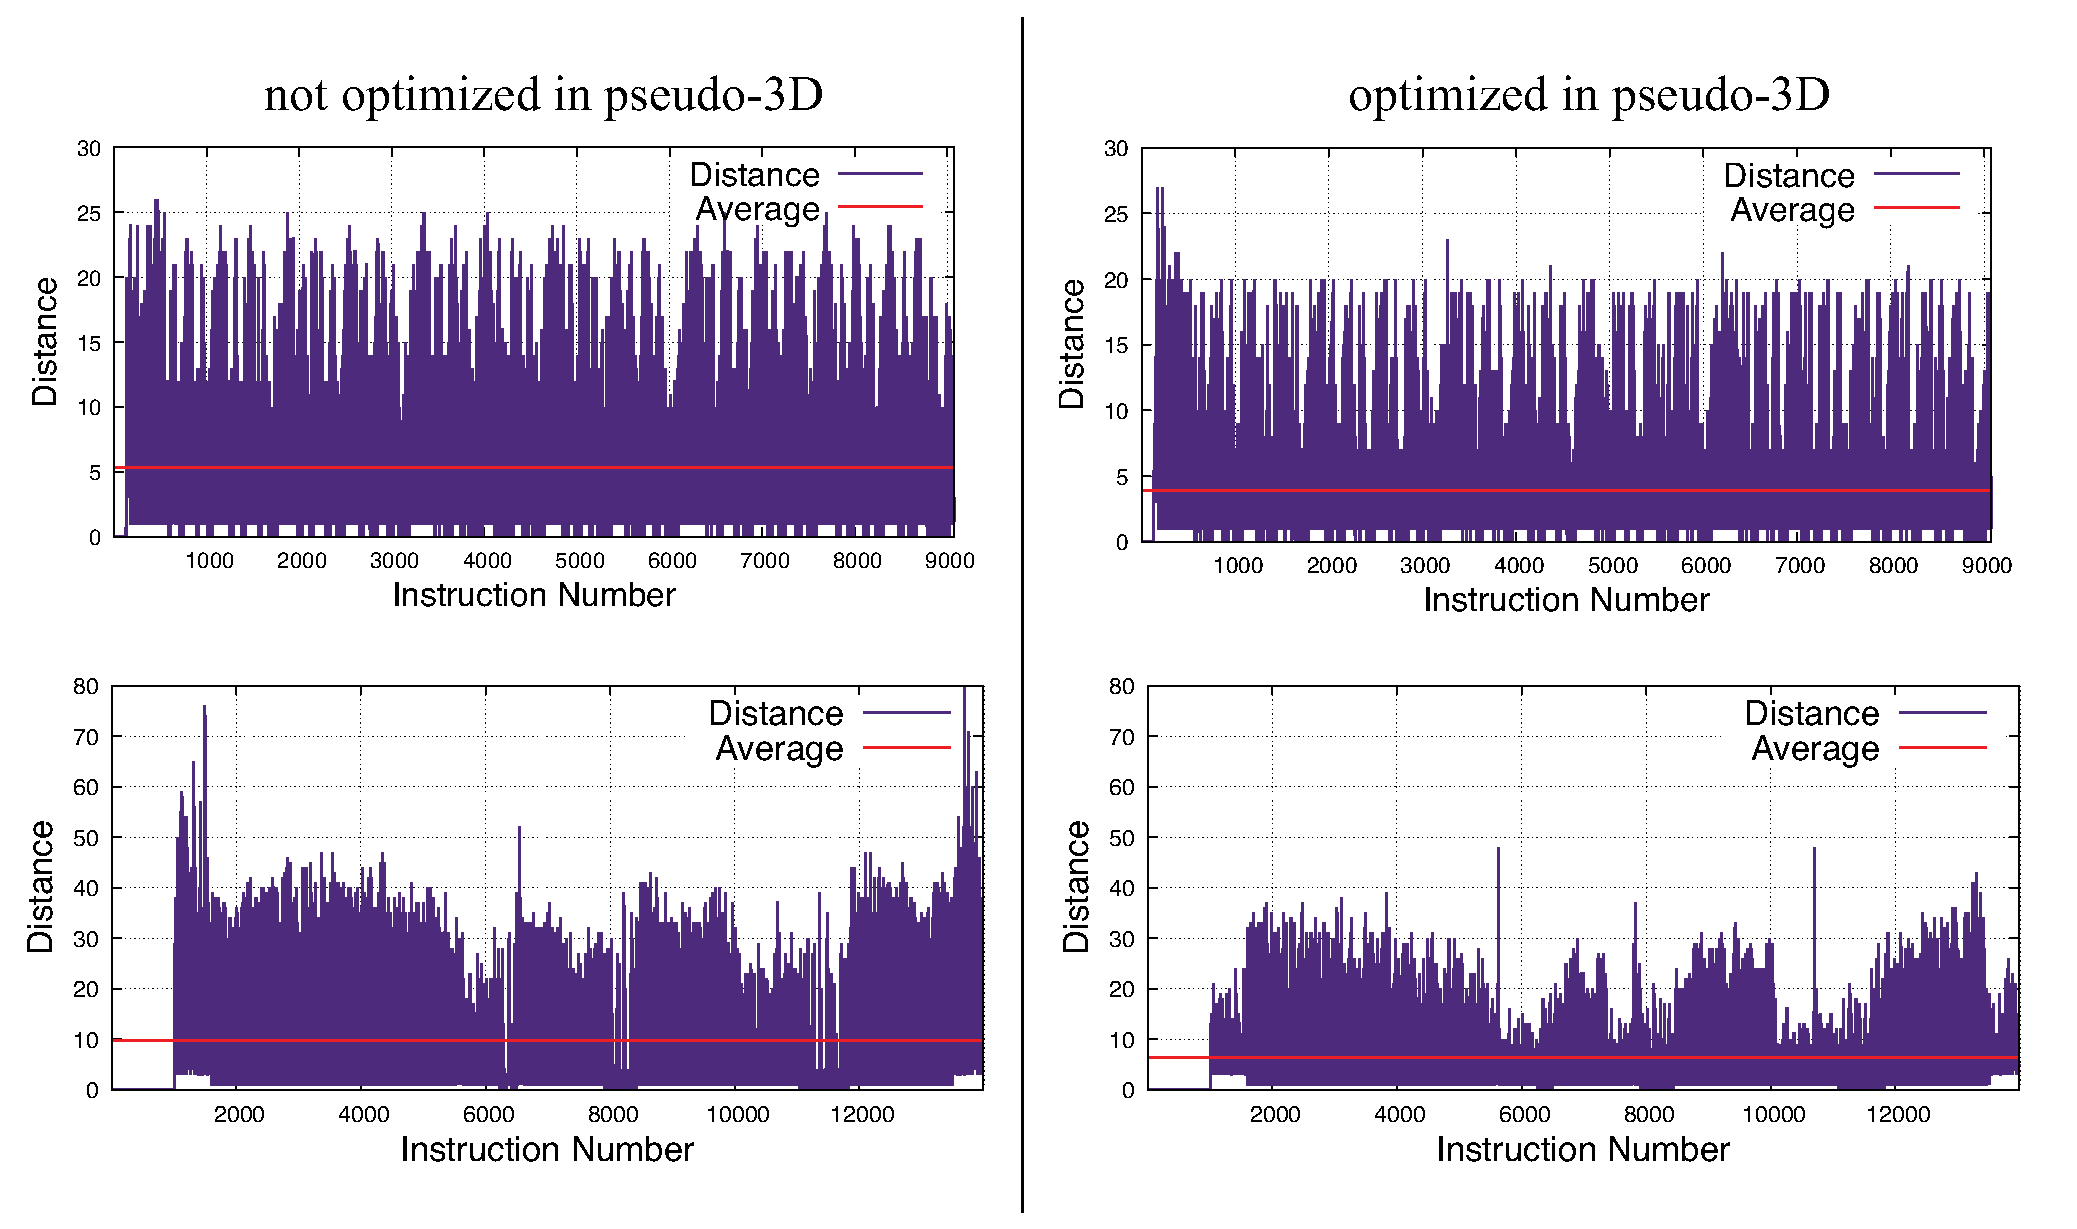
\includegraphics[scale=0.5]{figure/placement_optimization_3D.eps}
        \vspace{-20pt}\caption{Results of placement optimization for executing the 2D Heisenberg model circuit. (Left) Unoptimized cases in pseudo-3D surface codes. (Right) Optimized cases in pseudo-3D surface codes. Additionally, the bottom rows present results for more complex circuits compared to the top rows. The average values are 5.36 (left top), 3.93 (right top), 9.74 (left bottom), and 6.28 (right bottom).}
        \label{placement_optimization_3D}
    \end{figure}

    \ \ \ Similarly, in Fig.~\ref{placement_optimization_3D}, we observed that placement optimization effectively decreases routing distances in the pseudo-3D configuration. Specifically, the average distance in the pseudo-3D optimized configuration was reduced to 3.93 for the smaller circuit and to 6.28 for the larger circuit, resulting in a 73\% improvement in the smaller circuit and a 64\% improvement in the larger circuit.\\
    \ \ \ Throughout the all results, the distances needed to routing is more effectively reduced in the larger cicuit than that in smaller circuit. But there exists a trade-off that the BFS algorithm is more complicated in pseudo-3D, thus the routing time cannot be ignored in a larger circuit in the pseudo-3D. Moreover, placement optimization time in a graph also cannot be ignored in a larger circuit in the pseudo-3D.
    \clearpage

    \begin{figure}[h]
        \centering
        \includegraphics[scale=0.50]{figure/graph_2D.eps}
        \vspace{0pt}\caption{Graph representation of patch placement for the 2D Heisenberg circuit within a 2D surface code. The lower graph illustrates a more complex circuit compared to the upper graph. The \texttt{MAGIC\_NODE} is fixed at the bottom left corner. Node labels correspond to the logical qubits in the circuit.}
        \label{graph_2D}
        \includegraphics[scale=0.50]{figure/graph_3D.eps}
        \vspace{-10pt}\caption{Graph representation of the placement of patches for the 2D Heisenberg circuit in a pseudo-3D surface code. The bottom graph depicts a more complex circuit than the top graph. The \texttt{MAGIC\_NODE} is fixed at coordinates $(-1, 0, 0)$. The names within the nodes correspond to the logical qubits in the circuit.}
        \label{graph_3D}
    \end{figure}
}

\end{document}